\chapter{Model Overview}
\section{Introduction}
This section details the governing equations used to simulate the \gls{sco2} jet. All models and equations described here are from \textit{PeleC} \cite{PeleC1, PeleC2}, a compressible hydrodynamics code for reacting flows that leverages \textit{AMReX} \cite{amrex1, amrex2, amrex3} for \gls{amr}. It also leverages the \textit{PelePhysics} library for complex physics, including chemical reactions, non-ideal \gls{eos}, and high fidelity transport models. As introduced previously, the compressible Navier-Stokes equations form the basis of the model along with the \gls{srk}. Here we also detail the filtering used in the \gls{les} and the \gls{smd} used to model the \gls{sgs} dynamics \cite{LES_Comp}. We also describe the transport and thermodynamic models used for incorporating into the system real fluid dynamics involving supercritical conditions. 


\section{Governing Equations}

We consider the three-dimensional compressible Navier-Stokes equations, presented here with Einstein notation:
\begin{subequations} \label{NSE_einstein}
\begin{align}
  \frac{\partial\rho}{\partial t} + \frac{\partial }{\partial x_j} \left( \rho u_j \right) &= 0,  \label{NSE_mass}\\
  \frac{\partial}{\partial t} \left( \rho u_i \right) + \frac{\partial}{\partial x_j} \left(\rho u_i u_j + p \delta_{ij} -\sigma_{ij} \right) &= 0,  \label{NSE_mom}\\
  \frac{\partial}{\partial t} \left( \rho E \right) + \frac{\partial}{\partial x_j} \big(\left( \rho E+p \right) u_j + q_j - \sigma_{ij} u_i\big) &= 0, \label{NSE_E}
\end{align}
\end{subequations}
where $\rho$ is the density, $u_j$ is the velocity for the $x_j$ direction, $p$ is the pressure, $E = e + \frac{u_i u_i}{2}$ is the total energy, $e $ is the internal energy, and $T$ is the temperature. Following the assumptions made for Newtonian fluids \cite{batchelor_2000}, the diffusive fluxes are
\begin{equation} \label{Transport}
  \sigma_{ij} = 2\mu S_{ij} - \frac{2}{3}\mu \delta_{ij} S_{kk}, \quad \quad
  q_j = -\lambda \frac{\partial T}{\partial x_j},
\end{equation}
where
$S_{ij} = \frac{1}{2}\left(\frac{\partial u_i}{\partial x_j} + \frac{\partial u_j}{\partial x_i} \right)$ is the strain-rate tensor, $\mu$ is the dynamic viscosity, and $\lambda$ is the thermal conductivity. Models regarding these two components are given in more detail in the next section. $\delta_{ij}$ here is the Kronecker delta. External forces such as gravity are not included in this study. The system is closed using the \gls{srk} \cite{SOAVE1972} to relate pressure, density, and temperature as follows:
\begin{equation} \label{SRK_eos}
\begin{aligned} 
	p &= \dfrac{RT}{V_m - b} - \dfrac{a \alpha}{V_m(V_m + b)}, \\
	a &= \dfrac{0.42747R^2T_c^2}{P_c}, \\
	b &= \dfrac{0.08664RT_c}{P_c}, \\
	\alpha &= \left( 1 + \left( 0.48508 + 1.55171 \omega - 0.15613 \omega^2 \right)\left( 1 - T_r^{0.5} \right) \right)^2,
\end{aligned}
\end{equation}
where $R$ is the ideal gas constant, $T_c$ and $P_c$ are the critical temperature and pressure of the species, respectively, $T_r = T/T_c$ is the reduced temperature given by the ratio of the absolute temperature to the critical temperature, $V_m$ is the molar volume of the species, and $\omega$ is the acentric factor of the species. All cases are run with a single species, that being \gls{co2}. 

\subsection{Filtered Navier-Stokes Equations}
To perform the \gls{les}, we consider the filtered compressible Navier-Stokes equations as implemented by Mart\'{i}n, Piomelli, and Candler \cite{LES_Comp}. Here we go through a brief derivation along with the main assumptions needed. First, applying the filtering operation from Equation \eqref{les_filtering} to Equations \eqref{NSE_einstein}, we get:
\begin{subequations} \label{NSE_filtered}
\begin{align}
  \frac{\partial\overline{\rho}}{\partial t} + \frac{\partial }{\partial x_j} \left( \overline{\rho u_j} \right) &= 0,  \label{mass_filtered} \\
  \frac{\partial}{\partial t} \left( \overline{\rho u_i }\right) + \frac{\partial}{\partial x_j} \left(\overline{\rho u_i u_j} + \overline{p }\delta_{ij} - \overline{\sigma_{ij}} \right) &= 0,  \label{mom_filtered} \\
  \frac{\partial}{\partial t} \left( \overline{\rho E} \right) + \frac{\partial}{\partial x_j} \big(\left( \overline{\rho Eu_j}+\overline{p u_j} \right) + \overline{q_j} - \overline{\sigma_{ij} u_i}\big) &= 0. \label{en_filtered}
\end{align}
\end{subequations}
In order to avoid having to model $\overline{\rho u_j} $ in the conservation of mass equation in \eqref{NSE_filtered}, Favre-filtering, $\widetilde{\cdot}  = \nicefrac{\overline{\rho~\cdot}}{\overline{\rho}}$, is also applied \cite{favre}. Additionally, the following two sets of assumptions are made regarding transport terms \cite{PIOMELLI202183}:
\begin{subequations} \label{trans_assumptions}
\begin{align}
\overline{\mu(T)S_{ij}} \simeq \mu(\widetilde{T})\widetilde{S_{ij}}, \quad \quad 
\overline{\lambda(T)\dfrac{\partial T}{\partial x_j}} \simeq \lambda(\widetilde{T})\dfrac{ \partial \widetilde{T}}{\partial x_j}, \label{trans_1}\\
\widetilde{\mu} = \mu(\widetilde{T}), \quad \quad \widetilde{\lambda} = \lambda(\widetilde{T}).\label{trans_2}
\end{align}
\end{subequations}
The assumptions in Equations \eqref{trans_assumptions} are common in the literature regarding \gls{les}, even though transport terms depend nonlinearly on temperature \cite{PIOMELLI202183}. Justification for this type of assumption can be made where if performing \gls{les} with coarse enough grid, molecular transport coefficients remain small compared to turbulent transport coefficients \cite{roberts2002turbulent}. Applying Equations \eqref{trans_assumptions} along with the Favre filter to Equations \eqref{NSE_filtered} yields the following:
\begin{equation} \label{NSE_favre_filtered}
\begin{split}
  \frac{\partial\overline{\rho}}{\partial t} + \frac{\partial }{\partial x_j} \left( \overline{\rho}\widetilde{ u_j} \right) = 0,  \\
  \frac{\partial}{\partial t} \left( \overline{\rho}\widetilde{ u_i }\right) + \frac{\partial}{\partial x_j} \left(\overline{\rho}\widetilde{ u_i u_j} + \overline{p }\delta_{ij} - \widetilde{\sigma_{ij}} \right) = 0,  \\
  \frac{\partial}{\partial t} \left( \overline{\rho}\widetilde{ E} \right) + \frac{\partial}{\partial x_j} \left(\left( \overline{\rho}\widetilde{ Eu_j}+\overline{p u_j} \right) + \widetilde{q_j} - \overline{\sigma_{ij} u_i}\right) = 0, 
\end{split}
\end{equation}
with filtered Equations \eqref{Transport} now given by: 
\begin{equation} \label{filtered_trans}
  \widetilde{\sigma_{ij}} = 2\widetilde{\mu}\widetilde{ S_{ij}} - \frac{2}{3}\widetilde{\mu} \delta_{ij} \widetilde{ S_{kk}}, \quad \quad
  \widetilde{q_j} = -\widetilde{\lambda} \frac{\partial \widetilde{T}}{\partial x_j}.
\end{equation}

Final simplifications to Equations \eqref{NSE_favre_filtered} come from the \gls{sgs} terms. The \gls{sgs} stress $\tau_{ij}$, \gls{sgs} heat flux $\mathcal{Q}_j$, \gls{sgs} turbulent diffusion $\nicefrac{\partial \mathcal{J}_j}{\partial x_j}$, and \gls{sgs} turbulent viscous diffusion $\nicefrac{\partial \mathcal{D}_j}{\partial x_j}$ are set through the following definitions \cite{LES_Comp}:
\begin{equation} \label{sgs_defs}
\begin{aligned}
\tau_{ij} &= \overline{\rho}\left(\widetilde{u_i u_j} - \widetilde{u_i}\widetilde{u_j} \right), \\
\mathcal{Q}_{j} &= \overline{\rho}\left(\widetilde{u_j T} - \widetilde{u_j}\widetilde{T} \right), \\
\mathcal{J}_{j} &= \overline{\rho}\left(\widetilde{u_j u_k u_k} - \widetilde{u_j}\widetilde{u_k u_k} \right), \\
\mathcal{D}_{j} &= \overline{\rho}\left(\widetilde{\sigma_{ij}u_i} - \widetilde{\sigma_{ij}}\widetilde{u_i} \right).
\end{aligned}
\end{equation} 
After substituting the appropriate pieces of Equations \eqref{sgs_defs} into the momentum and energy components of \eqref{NSE_favre_filtered} and applying a few further assumptions, we eventually get the following:
\begin{subequations} \label{NSE_w_SGS}
\begin{align}
  \frac{\partial\overline{\rho}}{\partial t} + \frac{\partial }{\partial x_j} \left( \overline{\rho}\widetilde{ u_j} \right) = 0, \label{NSE_mass_sgs} \\
  \frac{\partial}{\partial t} \left( \overline{\rho}\widetilde{ u_i }\right) + \frac{\partial}{\partial x_j} \left(\overline{\rho}\widetilde{ u_i} \widetilde{u_j} + \overline{p }\delta_{ij} - \widetilde{\sigma_{ij}} \right) = - \frac{\partial \tau_{ij}}{\partial x_j}, \label{NSE_mom_sgs}  \\
  \frac{\partial}{\partial t} \left( \overline{\rho}\widetilde{ E} \right) + \frac{\partial}{\partial x_j} \left(\left( \overline{\rho}\widetilde{ E}+\overline{p} \right)\widetilde{u_j} + \widetilde{q_j} - \widetilde{\sigma_{ij}}\widetilde{ u_i}\right) = - \frac{\partial}{\partial x_j } \left( \gamma c_v \mathcal{Q}_j + \dfrac{1}{2} \mathcal{J}_j - \mathcal{D}_j \right),  \label{NSE_E_sgs}
\end{align}
\end{subequations}
with $\gamma = \nicefrac{c_p}{c_v}$. The simplification above hinges upon relating enthalpy to internal energy and pressure as in the ideal gas case with $h = e ~+~ \nicefrac{p}{\rho} = c_p T$ with $c_p$ assumed to be constant. Neither of these assumptions is consistent with supercritical fluids but is chosen here for ease of splitting Equations \eqref{NSE_w_SGS} into simulated vs.\ modeled quantities. This is also standard practice in many supercritical \gls{les} studies \cite{Same_LES, ALKANDARI2022122949, PETIT201361}, though these assumptions leave room for future work on incorporating higher order \gls{eos} into the \gls{les} derivation. 

Finally, it is also noted that the divergence of the \gls{sgs} heat flux and the \gls{sgs} turbulent diffusion are of comparable order of magnitude while the \gls{sgs} viscous diffusion is an order of magnitude smaller \cite{LES_Comp}. Therefore, the \gls{sgs} turbulent viscous diffusion is omitted from the system. The final set of equations to be discretized and advanced is:  
\begin{subequations} \label{filtered_NSE_FINAL}
\begin{align}
  \frac{\partial\overline{\rho}}{\partial t} + \frac{\partial }{\partial x_j} \left( \overline{\rho}\widetilde{ u_j} \right) = 0, \label{NSE_mass_FINAL} \\
  \frac{\partial}{\partial t} \left( \overline{\rho}\widetilde{ u_i }\right) + \frac{\partial}{\partial x_j} \left(\overline{\rho}\widetilde{ u_i} \widetilde{u_j} + \overline{p }\delta_{ij} - \widetilde{\sigma_{ij}} \right) = - \frac{\partial \tau_{ij}}{\partial x_j}, \label{NSE_mom_FINAL}  \\
  \frac{\partial}{\partial t} \left( \overline{\rho}\widetilde{ E} \right) + \frac{\partial}{\partial x_j} \left(\left( \overline{\rho}\widetilde{ E}+\overline{p} \right)\widetilde{u_j} + \widetilde{q_j} - \widetilde{\sigma_{ij}}\widetilde{ u_i}\right) = - \frac{\partial}{\partial x_j } \left( \gamma c_v \mathcal{Q}_j + \dfrac{1}{2} \mathcal{J}_j \right),  \label{NSE_E_FINAL}
\end{align}
\end{subequations}
with Equations \eqref{filtered_trans} describing the filtered transport coefficients. The \gls{sgs} stress $\tau_{ij}$, \gls{sgs} heat flux $\mathcal{Q}_{j}$, and \gls{sgs} turbulent diffusion $\mathcal{J}_j$ need to be modeled in order to close the system. 

While Equations \eqref{filtered_NSE_FINAL} are the equations discretized within \textit{PeleC}, in practice, we evolve these filtered quantities without explicitly filtering the solution. Here, the grid serves as the main filter for the \gls{les} while the specific box filter described in the next section is used to determine model coefficients. 


\subsection{Subgrid-Scale Modeling for Large Eddy Simulation}
We use the \gls{smd} \gls{les} model for compressible flow as described by Mart\'{i}n, Piomelli, and Candler \cite{LES_Comp}. In this work, the grid provides the implicit filtering of the equations. The \gls{sgs} stress tensor, $\tau_{ij}$, is included in the diffusive fluxes and is calculated as follows:
\begin{equation}
\begin{aligned}
	\tau_{ij} - \dfrac{\delta_{ij}}{3}\tau_{kk} &= -C_s^22\overline{\Delta}^2 \overline{\rho} |\widetilde{S}| \left( \widetilde{S}_{ij} - \dfrac{\delta_{ij}}{3} \widetilde{S}_{kk} \right) = C_s^2 \alpha_{ij},  \\
	 \tau_{kk} &= C_I 2\overline{\rho} \overline{\Delta}^2 |\widetilde{S}|^2 = C_I \alpha,
\end{aligned}
\end{equation}
with $\overline{\Delta}$ being the filter width associated with the smallest scale retained by the filtering operation ($\overline{\Delta}$ is the grid spacing for our cases). Additionally, $|\widetilde{S}| = (2\widetilde{S}_{ij}\widetilde{S}_{ij})^{1/2}$. The two model coefficients are calculated as follows:
\begin{equation} \label{smd_coeffs}
\begin{aligned}
	C = C_s^2 = \dfrac{\langle \mathcal{L}_{ij} M_{ij} \rangle}{\langle M_{kl}M_{kl} \rangle}, \quad \quad C_I = \dfrac{ \langle \mathcal{L}_{kk} \rangle}{\langle \beta - \widehat{\alpha} \rangle},
\end{aligned}
\end{equation}
where the Germano identity, $\mathcal{L}_{ij} = T_{ij} - \widehat{\tau}_{ij}$, is used to relate the \gls{sgs} stress tensor to the ``resolved turbulent stresses'', $\mathcal{L}_{ij} = \left( \overline{\rho u_i} \widehat{ \hspace{1.5pt} \overline{\rho u_j}}/\overline{\rho} \right) - \widehat{ \overline{\rho u_i}} \hspace{1.5pt} \widehat{\overline{\rho u_j}}/\widehat{\overline{\rho}}$, and the subtest stresses, $T_{ij} = \widehat{\overline{\rho}} \breve{\widetilde{u_i u_j}} - \widehat{\overline{\rho}} \breve{\widetilde{u_i}} \breve{\widetilde{u_j}}$ \cite{germano}. In this relationship, a hat denotes quantities associated with a test filter $\widehat{G}$ which has a characteristic length of $\widehat{\Delta}$. The breve denotes Favre-filtered quantities using $\widehat{G}$ (i.e., $\breve{\widetilde{f}} = \nicefrac{\widehat{\overline{\rho f}}}{\widehat{\overline{\rho}}}$). Additionally, $M_{ij} = \beta_{ij} - \widehat{\alpha_{ij}}$ with $\beta_{ij} = -2\widehat{\Delta}^2 \widehat{\overline{\rho}} |\breve{\widetilde{S}}| \left( \breve{\widetilde{S}}_{ij} - \delta_{ij} \breve{\widetilde{S}}_{kk}/3  \right)$ and $\beta = 2 \widehat{\Delta}^2  \widehat{\overline{\rho}} |\breve{\widetilde{S}}|^2 $. 


The \gls{sgs} heat flux $\mathcal{Q}_j$ is also modeled dynamically as in \cite{LES_Comp}:
\begin{equation} \label{sgs_heat_flux}
\mathcal{Q}_j = - \dfrac{\overline{\rho}\nu_T}{Pr_T} \dfrac{\partial \widetilde{T}}{\partial x_j} = - C\dfrac{\overline{\Delta}^2 \overline{\rho}  |\widetilde{S}|}{Pr_T} \dfrac{\partial \widetilde{T}}{\partial x_j},
\end{equation}
where $C$ is modeled as in Equation \eqref{smd_coeffs} and the turbulent Prandtl number, $Pr_\text{T}$, is calculated dynamically as:
\begin{equation}
\begin{aligned}
	Pr_\text{T} = \dfrac{C \langle T_k T_k  \rangle}{\langle \mathcal{K}_j T_j \rangle},
\end{aligned}
\end{equation}
where 
\begin{equation} \label{smd_other}
\begin{aligned}
	T_j = - \widehat{\Delta}^2  \widehat{\overline{\rho}} |\breve{\widetilde{S}}| \dfrac{\partial \breve{\widetilde{T}}}{\partial x_j} +  \overline{\Delta}^2  \overline{\rho} \widehat{|\widetilde{S}| \dfrac{\partial \widetilde{T}}{\partial x_j}}, \qquad \qquad \mathcal{K}_j = \left( \dfrac{ \widehat{\overline{\rho u_j} \overline{\rho T}}}{\overline{\rho}} \right) - \dfrac{ \widehat{\overline{\rho u_j}} \widehat{ \overline{\rho T}}}{\widehat{\overline{\rho}}}.
\end{aligned}
\end{equation}

Finally, the \gls{sgs} turbulent diffusion $\mathcal{J}_j$ is modeled following the strategy proposed by Knight et al.\ \cite{knight}:
\begin{equation} \label{sgs_turb_diff}
\mathcal{J}_j = \widetilde{u}_k \tau_{jk}
\end{equation}

For our simulations, we implement the three point box filter as described in \cite{filter} with a filter-grid ratio of 2, i.e.\  $\widehat{\Delta}=2\overline{\Delta}$. With this filter, the convolution kernel from Equation \eqref{les_filtering} is defined as follows: 
\begin{equation} \label{LES_cont_filter}
G(\vb{x} - \vb{r}) = 
\begin{cases} 
      \dfrac{1}{\widehat{\Delta}} & |\vb{x} - \vb{r}|\leq \dfrac{\widehat{\Delta}}{2}, \vspace{2pt}\\ 
      0 & \text{otherwise}.
   \end{cases}
\end{equation}
A discretized form of Equation \eqref{LES_cont_filter} is needed for the test filter in calculating the \gls{smd} model coefficients. \textit{PeleC} contains a variety of filtering options. In one dimension, this discretization results in the following implementation:
\begin{equation}
\overline{\phi}_i = \dfrac{1}{24}\epsilon^2\left(\phi_{i+1} + \phi_{i-1} \right) + \dfrac{1}{12}\left( 12 - \epsilon^2\right)\phi_i \quad i = 1,2,...,N,
\end{equation}
where $\epsilon$ is the grid filter ratio, which in our case is equal to two. Additionally, the subscript $i$ represents a given grid cell for $N$ discretized cells. This filter is used for any of the quantities containing a hat or breve as defined above in Equations \eqref{smd_coeffs}, \eqref{smd_other}, and \eqref{sgs_turb_diff}.

As noted previously, the choice of \gls{sgs} modeling is important to accurately capture the turbulence statistics of the system. M\"{u}ller et al.\ found that while the choice in thermodynamic modeling is crucial in capturing first-order moments, the effects \gls{sgs} modeling is limited to second-order moments \cite{doi:10.1063/1.4937948}. Therefore, our conclusions relating to the turbulence dynamics will be unaffected. That being said, \cite{doi:10.1063/1.4937948} also notes that the choice in \gls{sgs} model and numerical flux discretization had a larger than expected effect on resolved Reynolds stress profiles. Specifically, the constant Smagorinsky model yielded decaying fluctuation magnitudes during early evolution, resulting in the transition to a fully turbulent mixing zone to start from lower turbulence levels. However, this did agree with the jet break-up location inferred from mean density profiles, which were shifted slightly downstream by comparison to other \gls{sgs} models. These relationships will be taken into consideration for this study as well and noted in the discussion of Reynolds stress profiles.


\section{Transport Models}
Modeling of transport coefficients is done through \textit{PelePhysics} \cite{PelePhysics}. There are three modeling options available in \textit{PelePhysics}; we use the \textit{Simple} model. The \textit{Simple} model approximates ideal gas transport coefficients using EGLib functions \cite{ERN1995105}, which have the following form:
\begin{equation} \label{EGLib}
\ln{(q_0)} = \sum\limits_{n=1}^{4} a_{q,n}\left( \ln{(T)}\right)^{n-1},
\end{equation}
where $q_0$ is the transport quantity of interest (either thermal conductivity $\lambda$ or viscosity $\mu$) and $a$ is the appropriate pre-calculated polynomial fit coefficient (see Table \ref{EGLibCoeffs}). Chung's high pressure correction for viscosity and thermal conductivity are included to account for real gas dynamics \cite{chung:1988}: 
\begin{equation} \label{chung_general}
q = q_k + q_p,
\end{equation}
where $q_k$ is the low-pressure gas transport quantity related to the ideal gas quantity $q_0$ and $q_p$ is the high-pressure deviation. 

For viscosity, these quantities are:
\begin{equation}
\begin{split}
\mu_k = \mu_0 \left( \dfrac{1}{G_2} + A_6 Y \right), \\ 
\mu_p = \left(\dfrac{\num{36.344e-6}(MT_c)^{1/2}}{V_c^{2/3}}\right)A_7Y^2G_2\exp(A_8 + \dfrac{A_9}{T^*} + \dfrac{A_{10}}{T^{*2}}), 
\end{split}
\end{equation}
where $M$ is the molecular weight, $V_c$ is the critical molar volume, $T^* = T/\epsilon_k$ is a dimensionless temperature scaling using the Lennard-Jones potential well depth \cite{LennardJones_1931}, $Y = (\rho V_c)/6$, and $G_1 = (1-0.5Y)/(1-Y)^3$, and $G_2 = \left\{A_1\left[   1-\exp(-A_4Y)\right]/Y + A_2G_1\exp(A_5Y) + A_3G_1 \right\}/(A_1A_4 + A_2 + A_3)$. The constants $A_{1-10}$ are linear functions calculated as follows: 
\begin{equation}
A_i = a_{i0} + a_{i1} \omega + a_{i2} \mu_r^4 + a_{i3} \kappa \quad i = 1,..., 10,
\end{equation} 
where $\mu_r$ is the reduced dipole moment of the species, $\kappa$ is the association factor of the species, and $a_{ij}$ are constants (see Table \ref{chung-aij}).  

Similarly, thermal conductivity components are given by: 
\begin{equation}
\begin{split}
\lambda_k = \lambda_0 \left( \dfrac{1}{H_2} + B_6 Y \right), \\ 
\lambda_p = \left(\dfrac{\num{3.039e-4}(T_c/M)^{1/2}}{V_c^{2/3}}\right)B_7Y^2H_2T_r^{1/2},
\end{split}
\end{equation}
where $H_2 = \left\{B_1\left[   1-\exp(-B_4Y)\right]/Y + B_2G_1\exp(B_5Y) + B_3G_1 \right\}/(B_1B_4 + B_2 + B_3)$ and $B_{1-7}$ are defined as: 
\begin{equation}
B_i = b_{i0} + b_{i1} \omega + b_{i2} \mu_r^4 + b_{i3} \kappa \quad i = 1,..., 7,
\end{equation}
where $b_{ij}$ are constants (see Table \ref{chung-bij}). All species-related constants mentioned in this section can also be found in Table \ref{transport-coeffs-other}. 

These high pressure corrections as derived and analyzed by Chung et al.\ show improved accuracy for approximating transport properties over a wide range of temperatures and pressures when compared to experimental data for a variety of species \cite{chung:1988}. 

\section{Thermodynamics and Related Quantities}
Modeling of thermodynamic quantities is also done through \textit{PelePhysics} \cite{PelePhysics}. In a similar fashion to Equation \eqref{chung_general}, thermodynamic properties can be broken up into an ideal gas component and a departure from ideal gas behavior:
\begin{equation} \label{thermo_general}
q(\phi) = q_{I}(\phi) + q_{D}(\phi),
\end{equation}
where $\phi$ is the appropriate combination of state variables involving temperature, specific volume, and pressure, $q_{I}$ is the ideal state component and $q_{D}$ is the departure component. These decompositions can be derived from fundamental thermodynamic relations \cite{batchelor_2000}. For example, change in internal energy can be written as follows:
\begin{equation} \label{thermo_example}
de = \left( \dfrac{\partial e}{\partial T} \right)_{V_m} dT + \left[ T \left( \dfrac{\partial p}{\partial T} \right)_{V_m} - p  \right] dV_m.
\end{equation}
Substituting in the appropriate partial derivative using the \gls{srk} and integrating from an ideal state reference point $(v_m,t)$ to general point far from ideal conditions $(V_m,T)$ yields:
\begin{equation}  \label{thermo_SRK_sub}
e(V_m,T) - e(v_m,t) =  e(v_m,T) - e(v_m,t) + a \left[ \alpha - T \dfrac{\partial \alpha}{\partial T} \right] \int\limits_{v_m}^{V_m} \dfrac{1}{V(V + b)}dV.
\end{equation}
Simplifying the left- and right-hand side of Equation \eqref{thermo_SRK_sub} and utilizing the choice of $v_m \to \infty$ for the ideal state volume \cite{poling2001properties}, we get:
\begin{equation} \label{thermo_simplify}
e(V_m,T) =  e(\infty,T) + a \left[ \alpha - T \dfrac{\partial \alpha}{\partial T} \right] \int\limits_{\infty}^{V_m} \dfrac{1}{V(V + b)}dV.
\end{equation}
Evaluating the integral in Equation \eqref{thermo_simplify}, we arrive at the final expression for the internal energy of the species described by the \gls{srk}: 
\begin{equation} \label{thermo_final}
e(V_m,T) =  e_I(T) + a \left[ T \dfrac{\partial \alpha}{\partial T} - \alpha \right] \dfrac{1}{b}\ln\left( 1 + \dfrac{b}{V_m} \right),
\end{equation}
where $e_I(T)=c_vT$ is the ideal internal energy which only depends on temperature and $e_D(V_m, T) = a \left[ T \tfrac{\partial \alpha}{\partial T} - \alpha \right] \tfrac{1}{b}\ln\left( 1 + \tfrac{b}{V_m} \right)$ is the departure function for the internal energy. A similar procedure can be done to arrive at the decomposed enthalpy equation involving \gls{srk}-specific quantities:
\begin{equation} \label{thermo_enthalpy}
h(V_m,T) = h_I(T) +  a \left[ T \dfrac{\partial \alpha}{\partial T} - \alpha \right] \dfrac{1}{b}\ln\left( 1 + \dfrac{b}{V_m} \right) + \dfrac{RTb}{V_m - b} - \dfrac{a \alpha}{V_m + b}.
\end{equation}
The departure function can be directly evaluated while the ideal gas portion must be approximated.

Ideal specific heat at constant volume scaled by the ideal gas constant $\nicefrac{c_{v_I}}{R}$ is approximated with NASA polynomial fits \cite{NASAPoly}. These polynomial fits have the following form:
\begin{equation} \label{NASA_poly}
\psi(T) = c_{\psi, 0} + c_{\psi, 1}T + c_{\psi, 2}T^2 + c_{\psi, 3}T^3 + c_{\psi, 4}T^4  + c_{\psi, 5}\dfrac{1}{T},
\end{equation}
where $c_{\psi,0-5}$ are species-specific constants for each quantity's polynomial fit (see Table \ref{NASA-Coeffs}). Other ideal gas quantities of interest can also be calculated in this form via integration, so that $\psi$ here can be either ideal internal energy $\nicefrac{e_I}{RT}$, specific heat at constant volume $\nicefrac{c_{v_I}}{R}$, or enthalpy $\nicefrac{h_I}{RT}$. 
The equations for additional thermodynamic quantities, such as constant volume and constant pressure specific heat, and useful derivatives involving the \gls{srk} can be found in Appendix \ref{SRK-Derives}. 

\section{Model Validation}
Here we compare some thermodynamic and transport quantities with highly accurate data from the NIST WebBook \cite{NIST} in order to quantify the error present in our model within the regime of interest. Figure \ref{NIST_quantities_compare} depicts constant-pressure specific heat, density, shear viscosity, and thermal conductivity across the parameter regime explored by the three cases noted in this work. Overall, quantities of interest depicted here follow the same general trends as the NIST data, but with larger discrepancies between the two noted near the pseudo-boiling region denoted by the peak in specific heat. Most of the largest error values can be found in the $314-330K$ range, which means modeling errors will have the largest impact on the pseudo-boiling case presented here. Table \ref{max_error} contains the largest percent errors for each quantity along with the temperature value of that peak error location. Future studies will explore methods of achieving higher accuracy in thermodynamic and transport modeling in this challenging parameter regime. Since general trends are still followed by the models, results from this study should still provide insight into this region.
\begin{figure}[H]
\begin{subfigure}{0.45\textwidth}
	\centering
	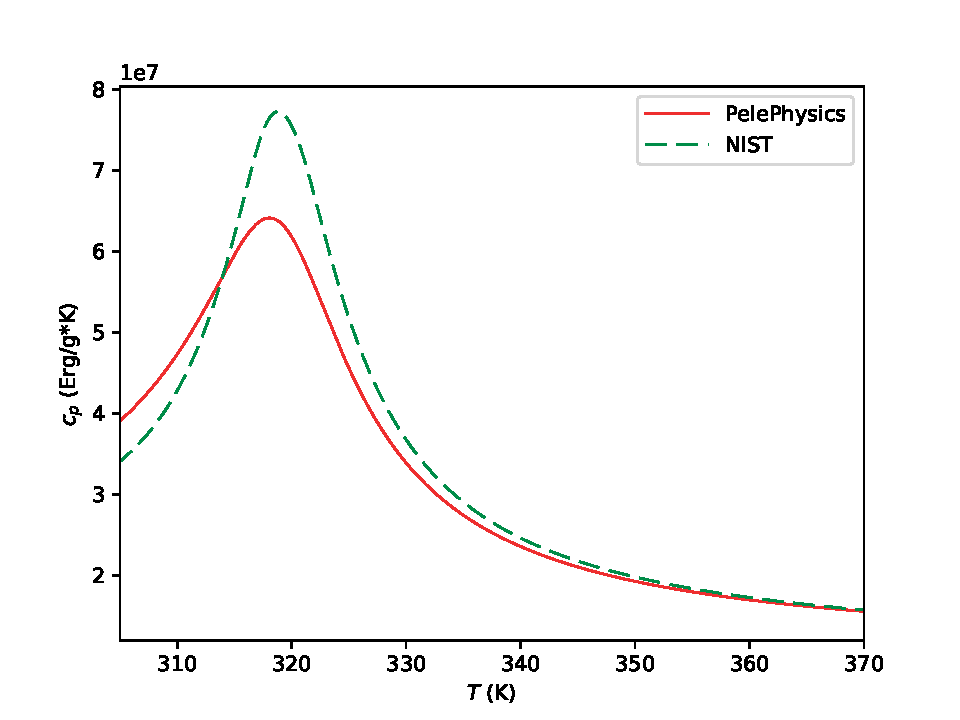
\includegraphics[scale=.45]{figures/Plots/NIST/cp_NIST_comp.pdf}
	\caption{Constant-Pressure Specific Heat across the temperature range of interest} \label{cp_NIST_comp}
\end{subfigure}
\hfill
\begin{subfigure}{0.45\textwidth}
	\centering
	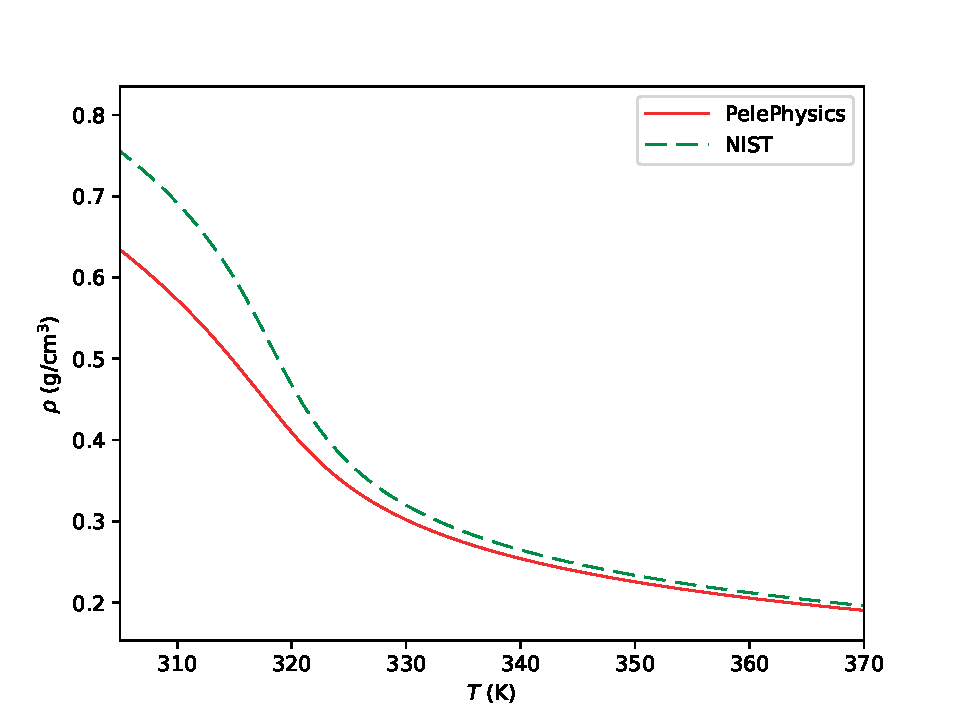
\includegraphics[scale=.45]{figures/Plots/NIST/rho_NIST_comp.pdf}
	\caption{Density across the temperature range of interest} \label{rho_NIST_comp}
\end{subfigure}
\vfill
\begin{subfigure}{0.45\textwidth}
	\centering
	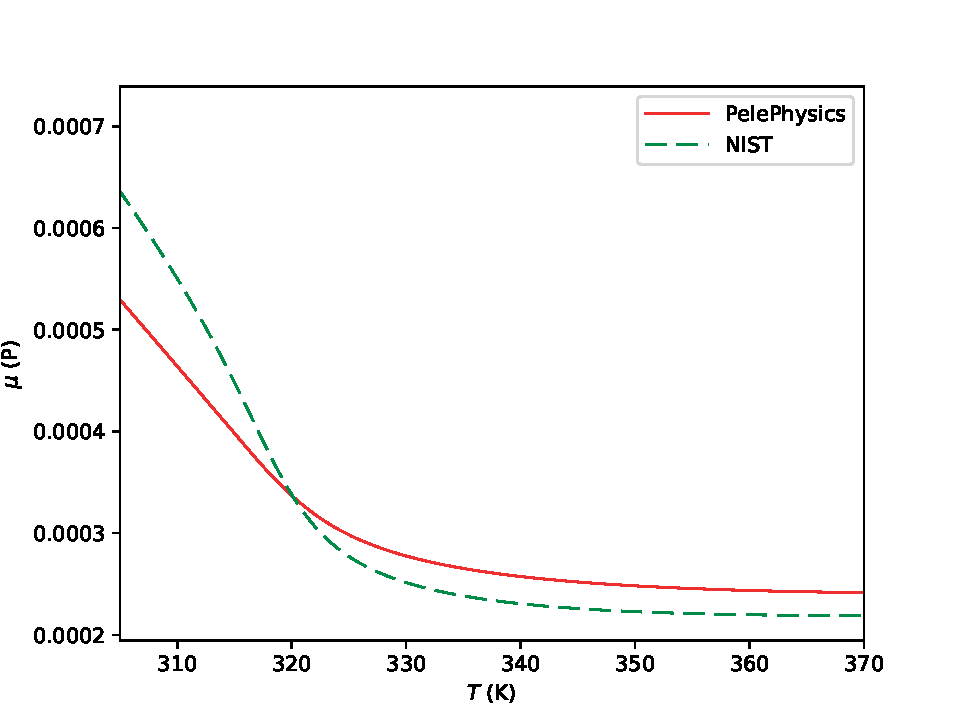
\includegraphics[scale=.45]{figures/Plots/NIST/mu_NIST_comp.pdf}
	\caption{Viscosity across the temperature range of interest} \label{mu_NIST_comp}
\end{subfigure}
\hfill
\begin{subfigure}{0.45\textwidth}
	\centering
	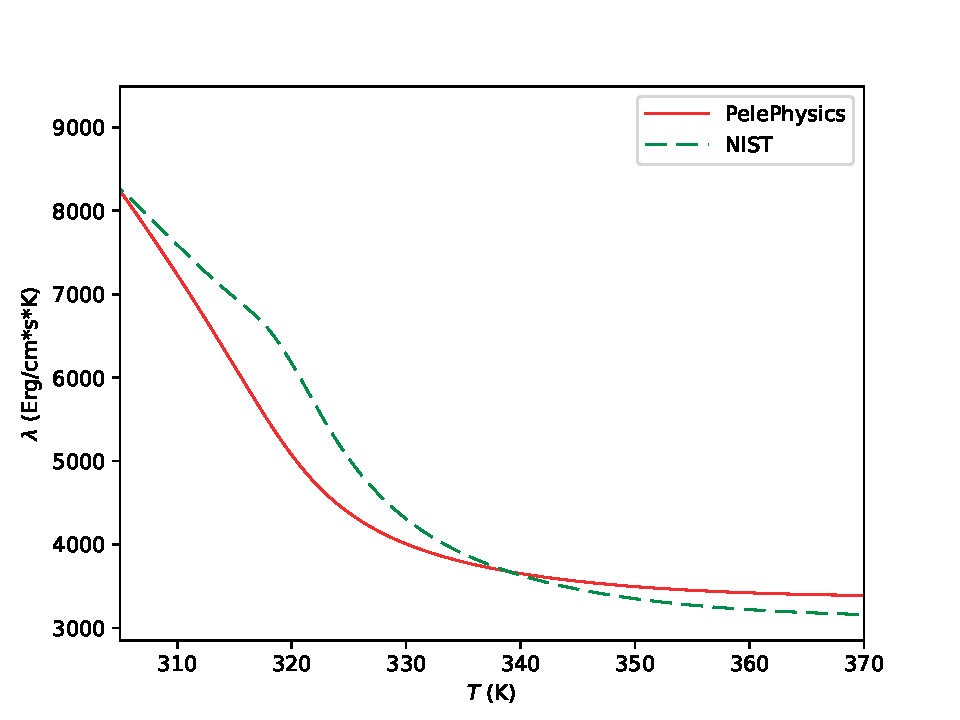
\includegraphics[scale=.45]{figures/Plots/NIST/lam_NIST_comp.pdf}
	\caption{Thermal Conductivity across the temperature range of interest} \label{lam_NIST_comp}
\end{subfigure}
\caption{Here we compare NIST WebBook values \cite{NIST} with output values from the thermodynamic and transport models described here as implemented in \textit{PelePhysics}. Challenges of capturing the fluid properties near the critical point can be seen in the increased error near the pseudo-boiling point near $318 K$.}
\label{NIST_quantities_compare}
\end{figure}

\begin{table}[H]
\caption{Maximum percent error between NIST WebBook Data and simulation models for constant-pressure specific heat, density, viscosity, and thermal conductivity.}
\label{max_error}
\begin{center}
\begin{tabular}{ r || r r }
Parameter & Percent Error & Temperature (K)  \\
\hline
$c_p$ & 18.11 & 320.25  \\
$\rho$ & 17.41 & 314  \\
$\mu$ & 12.62 & 314  \\
$\lambda$ & 17.81 & 319.88  \\

\end{tabular}
\end{center}
\end{table}



